%%%%%%%%%%%%%%%%%%%%%%%%%%%%%%%%%%%%%%%%%%%%%%%%%%%%%%%%%%%%%%%%%%%%%%%%%%%%%%%
\chapter{Diagonal Circulant Neural Networks}
\label{chapter:ch4-diagonal_circulant_neural_network}
%%%%%%%%%%%%%%%%%%%%%%%%%%%%%%%%%%%%%%%%%%%%%%%%%%%%%%%%%%%%%%%%%%%%%%%%%%%%%%%
\localtoc

% \begin{abstract}
% In this paper, we study deep diagonal circulant neural networks, which are deep neural networks in which weight matrices are the product of diagonal and circulant ones.
% Besides making a theoretical analysis of their expressivity, we introduce principled techniques for training these models: we devise an initialization scheme and propose a smart use of non-linearity functions in order to train deep diagonal circulant networks. 
% Furthermore, we show that these networks outperform recently introduced deep networks with other types of structured layers. We conduct a thorough experimental study to compare the performance of deep diagonal circulant networks with state-of-the-art models based on structured matrices and with dense models. We show that our models achieve better accuracy than other structured approaches while requiring 2x fewer weights than the next best approach. Finally, we train compact and accurate deep diagonal circulant networks on a real world video classification dataset with over 3.8 million training examples. 
% \end{abstract}

%%%%%%%%%%%%%%%%%%%%%%%%%%%%%%%%%%%%%%%%%%%%%%%%%%%%%%%%%%%%%%%%%%%%%%%%%%%%%%%%
\section{Introduction}
\label{chapter:p1-ch4_introduction}
%%%%%%%%%%%%%%%%%%%%%%%%%%%%%%%%%%%%%%%%%%%%%%%%%%%%%%%%%%%%%%%%%%%%%%%%%%%%%%%%

In this chapter, we study deep diagonal circulant neural networks, which are deep neural networks in which weight matrices are the product of diagonal and circulant ones.
We provide deep diagonal circulant neural networks with strong theoretical guarantees by showing that these networks with $\relu$ activations, limited width and shallow depth can approximate any dense neural network with arbitrary precision.
More precisely, we prove that for a deep ReLU network, $\nn$ of width $n$ and depth $l$ built from weight matrices $\Wmat^{(i)}$ of rank $k_i$, there exists a diagonal circulant ReLU network $\dcnn$ of width $n$ and of depth $9(\sum_i^l k_i)$ approximating $\nn$ with arbitrary precision, under some technical conditions.
To demonstrate this, we first need to prove that any matrix of rank $k$ can be approximated by an alternating product of $O(k)$ circulant and diagonal matrices.
This result improves the one of \citet{huhtanen2015factoring}, and constitutes the cornerstone of our theoretical analysis.
Indeed, it helps us demonstrate that the class of functions represented by bounded depth circulant networks is a strict superset of the class of functions represented by dense networks whose sum of ranks ($\sum k_i$) is bounded.
This means that any dense network whose sum of ranks is bounded can be approximated by a bounded-depth circulant network, but the converse is not true.
To sum up, the contributions of the chapter are the following.
\begin{enumerate}
  \item We conduct a theoretical analysis to provide deep -- fully structured -- circulant networks with strong theoretical guarantees regarding their expressivity.
  \item We describe a theoretically sound initialization procedure for these networks which simplifies their training and removes a large number of complex hyperparameters. 
  \item We provide a number of empirical insights to explain the behavior of deep fully circulant networks.
    More specifically, we show the impact of the number of non-linearities in the network on the convergence rate and the final accuracy of the network.
    We also show that it is easy to control the accuracy for the number of factors in the matrix decomposition, and hence the model size.
\end{enumerate}
The chapter is organized as follows:
Section~\ref{section:p1-ch4-a_primer_on_circulant_matrices_and_a_new_result} introduces our new result extending the one from \citet{huhtanen2015factoring}.
Section~\ref{section:p1-ch4-analysis_of_diagonal_circulant_neural_networks} proposes a theoretical analysis on the expressivity on DCNNs.
Section~\ref{section:p1-ch4-how_to_train_deep_diagonal_circulant_neural_networks} describes two efficient techniques for training deep diagonal circulant neural networks.
Finally, Section~\ref{section:p1-ch4-experiments} presents extensive experiments to compare the performance of deep diagonal circulant neural networks in different settings with respect to other state of the art approaches.


%%%%%%%%%%%%%%%%%%%%%%%%%%%%%%%%%%%%%%%%%%%%%%%%%%%%%%%%%%%%%%%%%%%%%%%%%%%%%%%
\section{A Primer on the Expressivity of Circulant Matrices and a New Result}
\label{section:p1-ch4-a_primer_on_circulant_matrices_and_a_new_result}
%%%%%%%%%%%%%%%%%%%%%%%%%%%%%%%%%%%%%%%%%%%%%%%%%%%%%%%%%%%%%%%%%%%%%%%%%%%%%%%

As seen in the Related Work (Chapter~\ref{chapter:p1-ch3-related_work}), circulant matrices exhibit several interesting properties from the perspective of numerical computations.
Most importantly, any $n \times n$ circulant matrix $\Cmat$ can be represented using only $n$ coefficients instead of the $n^2$ coefficients required to represent classical unstructured matrices.
In addition, the matrix-vector product is simplified from $O(n^2)$ to $O(n \log n)$ using the  convolution theorem.
As we will show in this chapter, circulant matrices also have a strong expressive power.
So far, we know that a single circulant matrix can be used to represent a variety of important linear transforms such as random projections~\cite{hinrichs2011johnson}. 
However, when they are combined with diagonal matrices, they can also be used as building blocks to represent any linear transform~\cite{schmid2000decomposing,huhtanen2015factoring} with an arbitrary precision.

First, we are interested in the relation between the product of diagonal and circulant matrices and low-rank matrices.
\citet{huhtanen2015factoring} were able to bound the number of factors that is required to approximate any matrix $\Amat$ with arbitrary precision.
We recall this result in Theorem~\ref{theorem:p1-ch4-huhtanen} as it is the starting point of our theoretical analysis.

\begin{theorem}[Reformulation from \citet{huhtanen2015factoring}]
  For every matrix $\Amat \in \Cnn$, for any $\epsilon > 0$, there exists a sequence of matrices $\Bmat^{(1)} \ldots \Bmat^{(2n-1)}$ where $\Bmat^{(i)}$ is a circulant matrix if $i$ is odd, and a diagonal matrix otherwise, such that $\norm{\Bmat^{(1)} \ldots \Bmat^{(2n-1)} - \Amat} < \epsilon$.
  \label{theorem:p1-ch4-huhtanen}
\end{theorem}

\noindent
Unfortunately, this theorem is of little use to understand the expressive power of diagonal-circulant matrices when they are used in deep neural networks for two reasons:
\begin{enumerate}
  \item the bound only depends on the dimension of the matrix $\Amat$, not on the matrix itself;
  \item the theorem does not provide any insights regarding the expressive power of $m$ diagonal-circulant factors when $m$ is much lower than $2n - 1$ as it is the case in most practical scenarios we consider in this chapter. 
\end{enumerate}

In the following theorem, we enhance the result of~\citet{huhtanen2015factoring} by expressing the number of factors required to approximate $\Amat$, \emph{as a function of the rank of $\Amat$}.
This is useful when one deals with low-rank matrices, which is common in machine learning problems. 
\begin{theorem}[Rank-based circulant decomposition]
  Let $\Amat \in \Cnn$ be a matrix of rank at most $k$.
  Assume that $n$ can be divided by $k$.
  For any $\epsilon > 0$, there exists a sequence of $4k+1$ matrices $\Bmat^{(1)} \ldots \Bmat^{(4k+1)}$, where $\Bmat^{(i)}$ is a circulant matrix if $i$ is odd, and a diagonal matrix otherwise, such that $\norm{\Bmat^{(1)} \ldots \Bmat^{(4k+1)} - \Amat} < \epsilon$.
  \label{theorem:p1-ch4-rank-decomposition}
\end{theorem}

\noindent
We defer the proof of Theorem~\ref{theorem:p1-ch4-rank-decomposition} in Appendix~\ref{chapter_appendix:technical_proofs}.
A direct consequence of Theorem~\ref{theorem:p1-ch4-rank-decomposition}, is that if the number of diagonal-circulant factors is set to a value $K$, we can represent all linear transform $\Amat$ whose rank is $\frac{K - 1}{4}$.
Compared to \citet{huhtanen2015factoring}, this result shows that structured matrices with fewer than $2n$ diagonal-circulant matrices (as it is the case in practice) can still represent a large class of matrices.
As we will show in the following section, this result will be useful to analyze the expressivity of neural networks based on diagonal and circulant matrices.


%%%%%%%%%%%%%%%%%%%%%%%%%%%%%%%%%%%%%%%%%%%%%%%%%%%%%%%%%%%%%%%%%%%%%%%%%%%%%%%
 \section{Analysis of Diagonal Circulant Neural Networks}
\label{section:p1-ch4-analysis_of_diagonal_circulant_neural_networks}
%%%%%%%%%%%%%%%%%%%%%%%%%%%%%%%%%%%%%%%%%%%%%%%%%%%%%%%%%%%%%%%%%%%%%%%%%%%%%%%

\citet{zhao2017theoretical} have shown that circulant networks with 2 layers and unbounded width are universal approximators.
However, results on unbounded networks offer weak guarantees and two important questions have remained open until now: 
\begin{enumerate}
  \item \emph{Can we approximate any function with a bounded-width diagonal-circulant networks?}
  \item \emph{What function can we approximate with a diagonal circulant neural network that has a bounded width and a small depth?}
\end{enumerate}
We answer these two questions in this section.
First, we introduce some technical but necessary definitions regarding neural networks and provide a theoretical analysis of their approximation capabilities.  

\begin{definition}[Complex ReLU function \citet{trabelsi2018deep}]
  Let us define the complex $\relu$ function $\rho: \Cn \rightarrow \Cn$ by: $\rho(\zvec) = \max\left(0, \mathfrak{R}(\zvec)\right) + \ci \max\left(0, \mathfrak{I}(\zvec) \right)$
  \label{definition:relu_function}
\end{definition}

\begin{definition}[Deep ReLU network] \label{definition:deep_relu_network}
  Given $L$ weight matrices $\Wmat = (\Wmat^{(1)}, \ldots, \Wmat^{(L)})$ with $\Wmat^{(i)} \in \Cnn$ and  $L$ bias vectors $\Bmat = (\bvec^{(1)}, \ldots, \bvec^{(L)})$  with  $\bvec^{(i)} \in \Cn$, a \emph{deep $\relu$ network} is a function $\nn_{\Wmat, \Bmat} : \Cn \rightarrow \Cn$ such that
  \begin{equation}
    \nn_{\Wmat,\Bmat}(\xvec) \triangleq \phi_{\Wmat^{(L)}, \bvec^{(L)}} \circ \cdots \circ \phi_{\Wmat^{(1)}, \bvec^{(1)}}(\xvec)
  \end{equation}
  where $\phi_{\Wmat^{(i)},\bvec^{(i)}} \triangleq \rho\left(\Wmat^{(i)}\xvec + \bvec^{(i)}\right)$ and $\rho$ is the $\relu$ function.
  In the rest of this chapter, we call $L$ and $n$ respectively the depth and the width of the network.
\end{definition}

\begin{definition}[Total Rank]
  The total rank $k$ of the neural network $f_{\Wmat, \Bmat}$ corresponds to the sum of the ranks of the matrices $\Wmat^{(1)} \ldots \Wmat^{(L)}$ \ie, $k = \sum_{i=1}^L \rank(\Wmat^{(i)})$.
\end{definition}

\noindent
We also need to formally define diagonal circulant neural network similarly to neural networks.

\begin{definition}[Diagonal Circulant Neural Networks] \label{definition:DCNN}
  Given $L$ diagonal matrices $\Dmat = (\Dmat^{(1)}, \ldots, \Dmat^{(L)})$ with $\Dmat^{(i)} \in \Cnn$, $L$ circulant matrices $\Cmat = (\Cmat^{(1)}, \ldots, \Cmat^{(L)})$ with $\Cmat^{(i)} \in \Cnn$ and $L$ bias vectors $\Bmat = (\bvec^{(1)}, \ldots, \bvec^{(L)})$ with  $\bvec^{(i)} \in \Cn$, a \emph{Diagonal Circulant Neural Networks (DCNN)} is a function $\dcnn_{\Dmat, \Cmat, \Bmat} : \Cn \rightarrow \Cn$ such that 
  \begin{equation}
    \dcnn_{\Dmat,\Cmat,\Bmat}(\xvec) = \phi_{\Dmat^{(L)}, \Cmat^{(L)}, \bvec^{(L)}} \circ \ldots \circ \phi_{\Dmat^{(1)}, \Cmat^{(1)}, \bvec^{(1)}} (\xvec)
  \end{equation}
   where $\phi_{\Dmat^{(i)}, \Cmat^{(i)}, \bvec^{(i)}}(\xvec) = \rho (\Dmat^{(i)} \Cmat^{(i)} \xvec + \bvec^{(i)})$ and where $\rho$ is the $\relu$ function.
\end{definition}


\noindent
We can now show that bounded-width DCNNs can approximate any Deep ReLU Network, and as a corollary, that they are universal approximators.

\begin{lemma}
  Let $\Wmat^{(L)} \ldots \Wmat^{(1)} \in \Cbb^{n\times n}$, $\bvec \in \Cn$ and let $\Xset \subset \Cn$ be a bounded set.
  There exists $\beta^{(L)} \ldots \beta^{(1)} \in \Cn$ such that for all $\xvec \in \Xset$ we have 
  \begin{equation}
    \rho\left(\Wmat^{(L)} \ldots \Wmat^{(1)}\xvec + \bvec \right) = \phi_{\Wmat^{(L)},\beta^{(L)}} \circ \ldots \circ \phi_{\Wmat^{(1)},\beta^{(1)}}(\xvec)
  \end{equation}
  \label{lemma:product_of_mat_to_DNN}
\end{lemma}

\begin{proof}[\proofreflem{lemma:product_of_mat_to_DNN}]
  Let is define
  \begin{equation}
    S = \left\{ \left(\left(\prod_{k=1}^{j} \Wmat^{(k)} \right) \xvec \right)_{t}: \xvec \in \Xset, t \in [n], j \in [L] \right\}
  \end{equation}
  and let $\Omega = \max\left\{ \mathfrak{R}(v): v \in S \right\} + \ci \max\left\{ \mathfrak{I}(v):v \in S \right\}$.
  Intuitively, the real and imaginary parts of $\Omega$ are the largest any activation in the network can have.
  Define $\psi^{(j)}(\xvec) = \Wmat^{(j)} \xvec + \beta^{(j)}$. Let $\beta^{(1)} = \Omega \vecones{n}$.
  Clearly, for all $\xvec \in \Xset$ we have $\psi^{(1)}(\xvec) \ge 0$, so $\rho\ \circ\ \psi^{(1)}(\xvec) = \psi^{(1)}(\xvec)$.
  More generally, for all $j < n-1$ define $\beta^{(j+1)} = \vecones{n} \Omega - \Wmat^{(j+1)} \beta^{(j)}$.
  It is easy to see that for all $j < n$ we have $\psi^{(j)} \circ \ldots \circ \psi^{(1)}(\xvec) = \Wmat^{(j)} \Wmat^{(j-1)} \ldots \Wmat^{(1)} \xvec + \vecones{n} \Omega$.
  This guarantees that for all $j < n$, $\psi^{(j)} \circ \ldots \circ \psi^{(1)}(\xvec) = \rho \circ \psi^{(j)} \circ \ldots \circ \rho  \circ \psi^{(1)}(\xvec)$.
  Finally, define $\beta^{(L)} = \bvec - \Wmat^{(L)} \beta^{(L-1)}$.
  We have,
  \begin{equation}
    \rho \circ \psi^{(L)} \circ \ldots \circ \rho \circ \psi^{(1)}(\xvec) = \rho \left(\Wmat^{(j)} \ldots \Wmat^{(1)} \xvec + \bvec \right) \enspace.
  \end{equation}
\end{proof}


\begin{lemma} \label{lemma:dcnn_approx_neural_network}
  Let $\nn$ be a deep ReLU network of width $n$ and depth $L$, and let $\Xset \subset \Cn$ be a bounded set.
  For any $\epsilon > 0$, there exists a diagonal circulant neural network $\dcnn$ of width $n$ and of depth $(2n-1)L$ such that $\norm{\nn(\xvec) - \dcnn(\xvec)} < \epsilon$ for all $\xvec \in \Xset$.
\end{lemma}

\begin{proof}[\proofreflem{lemma:dcnn_approx_neural_network}]
  Let us assume $\nn = \phi_{\Wmat^{(L)}, \bvec^{(L)}} \circ \ldots \circ \phi_{\Wmat^{(1)}, \bvec^{(1)}}$.
  By Theorem~\ref{theorem:p1-ch4-huhtanen}, for any $\epsilon' > 0$, any matrix $\Wmat^{(i)}$, there exists a sequence of $2n-1$ matrices $\Cmat^{(i,n)} \Dmat^{(i,n-1)} \ldots \Dmat^{(i,1)} \Cmat^{(i,1)}$ such that 
  \begin{equation}
    \norm{\prod_{j=0}^{n-1} \Dmat^{(i,n-j)} \Cmat^{(i,n-j)} - \Wmat^{(i)}} < \epsilon' , 
  \end{equation}
  where $\Dmat^{(i,1)}$ is the identity matrix.
  By Lemma~\ref{lemma:product_of_mat_to_DNN}, we know that there exists $\left\{ \beta^{(i,j)} \right\}_{i \in[L], j \in [n]}$ such that for all $i\in[L]$, 
  \begin{equation}
    \phi_{\Dmat^{(i,n)} \Cmat^{(i, n)}, \beta^{(i, n)}} \circ \ldots \circ \phi_{\Dmat^{(i,1)} \Cmat^{(i, 1)}, \beta^{(i, 1)}}(\xvec) = \rho \left(\Dmat^{(i,n)} \Cmat^{(i,n)} \ldots \Cmat^{(i,1)} \xvec + \bvec^{(i)} \right).
  \end{equation}
  Now if $\epsilon'$ tends to zero, $\norm{ \phi_{\Dmat^{(i,n)} \Cmat^{(i,n)},\beta^{(i,n)}} \circ \ldots \circ \phi_{\Dmat^{(i,1)}, \Cmat^{(i,1)}, \beta^{(i,1)}} - \rho \left(\Wmat^{(i)} \xvec + \bvec^{(i)} \right)}$ will also tend to zero for any $\xvec \in \Xset$, because the ReLU function is continuous and $\Xset$ is bounded.
  Let $f' = \phi_{\Dmat^{(1,n)} \Cmat^{(1,n)},\beta^{(1,n)}} \circ \ldots \circ \phi_{\Dmat^{(i,1)}, \Cmat^{(i,1)}, \beta^{(i,1)}}$, because all functions are continuous, for all $\xvec \in \Xset$, $\norm{ f(\xvec) - f'(\xvec)} $ tends to zero as $\epsilon'$ tends to zero.
\end{proof}


\noindent
With the help of Lemma~\ref{lemma:dcnn_approx_neural_network}, we can now state the universal approximation corollary:

\begin{corollary} \label{corollary:universal}
  % Bounded width DCNNs are universal approximators in the following sense: 
  Diagonal circulant neural networks with bounded width are universal approximators in the following sense:
  for any continuous function $g:[0,1]^{n} \rightarrow \Rbb_+$ of bounded supremum norm, for any $\epsilon > 0$, there exists a diagonal circulant neural network $f_{\epsilon}$ of width $n+3$ such that $\forall \xvec \in [0,1]^{n+3}$, $\left| g(\xvec_{1} \ldots \xvec_{n}) - \left( f_{\epsilon} \left( \xvec \right) \right)_{1} \right| < \epsilon$, where $\left(\ \cdot\ \right)_{i}$ represents the $i^{th}$ component of a vector.
\end{corollary}


\begin{proof}[\proofrefcor{corollary:universal}]
It has been shown recently by~\citet{hanin2017universal} that for any continuous function $f:[0,1]^{n} \rightarrow \mathbb{R}_+$ of bounded supremum norm, for any $\epsilon>0$, there exists a dense neural network $\mathcal{N}$ with an input layer of width $n$, an output layer of width $1$, hidden layers of width $n+3$ and ReLU activations such that $\forall x \in [0,1]^n, \left| f(\xvec) - \mathcal{N} \left(\xvec\right)\right| < \epsilon$. From $\mathcal{N}$, we can easily build a deep ReLU network $\mathcal{N'}$ of width exactly $n+3$, such that $\forall x \in [0,1]^{n+3}$, $\left|f(\xvec_{1} \ldots \xvec_{n}) - \left(\mathcal{N}'\left(\xvec\right)\right)_{1}\right| < \epsilon$. Thanks to Lemma~\ref{lemma:dcnn_approx_neural_network}, this last network can be approximated arbitrarily well by a DCNN of width $n+3$.
\end{proof}


This is a first result, however $(2n+5)L$ is not a small depth (in our experiments, $n$ can be over 300~000), and a number of work provided empirical evidences that DCNN with small depth can offer good performances \cite{araujo2018training,cheng2015exploration}.
To improve our result, we introduce our main theorem which studies the approximation properties of these small depth networks.

\begin{theorem}[Rank-based expressive power of DCNNs] \label{theorem:p1-ch4-low_rank_nn}
  Let $\mathcal{N}$ be a deep ReLU network of width $n$, depth $L$ and a total rank $k$ and assume $n$ is a power of $2$.
  Let $\Xset \subset \Cn$ be a bounded set.
  Then, for any $\epsilon > 0$, there exists a DCNN with ReLU activation $\mathcal{N}'$ of width $n$ such that $\norm{ \mathcal{N}(\xvec) - \mathcal{N}'(\xvec)} < \epsilon$ for all $\xvec \in \Xset$ and the depth of $\mathcal{N}'$ is bounded by $9k$.
\end{theorem}

\begin{proof}[\proofrefth{theorem:p1-ch4-low_rank_nn}]
  Let $k_{1} \ldots k_{L}$ be the ranks of matrices $\Wmat^{(1)} \ldots \Wmat^{(L)}$, which are $n$-by-$n$ matrices.
  For all $i$, there exists $k_{i}' \in \{k_{i} \ldots 2k_{i}\}$ such that $k'_{i}$ is a power of $2$.
  Due to the fact that $n$ is also a power of $2$, $k'_{i}$ divides $n$.
  By Theorem~\ref{theorem:p1-ch4-rank-decomposition}, for all $i$ each matrix $\Wmat^{(i)}$ can be decomposed as an alternating product of diagonal-circulant matrices $\Bmat_{i,1} \ldots \Bmat_{i,4k'_{i}+1}$ such that $\norm{ \Wmat^{(i)} - \Bmat_{i,1} \ldots \Bmat_{i,4k'_{i}+1}} < \epsilon$.
  Using the exact same technique as in Lemma~\ref{lemma:dcnn_approx_neural_network}, we can build a DCNN $\mathcal{N}'$ using matrices $\Bmat_{1,1} \ldots \Bmat_{L,4k'_{L}+1}$, such that $\norm{ \mathcal{N}(\xvec) - \mathcal{N}'(\xvec)} < \epsilon$ for all $\xvec \in \Xset$.
  The total number of layers is $\sum_{i}\left(4k_{i}'+1\right)\le L+8\sum_{i}k_{i}\le L+8.
  \textrm{total rank} \le 9.\textrm{total rank}$.
\end{proof}

Remark that in the theorem, we require that $n$ is a power of $2$.
We conjecture that the result still holds even without this condition.
This result refines Lemma~\ref{lemma:dcnn_approx_neural_network}, and answer our second question: a DCNN of bounded width and small depth can approximate a Deep ReLU network of low  total rank.
Note that the converse is not true: because $n$-by-$n$ circulant matrix can be of rank $n$, approximating a DCNN of depth $1$ can require a deep ReLU network of total rank equals to $n$.


Finally, what if we choose to use small depth networks to approximate deep ReLU networks where matrices are not of low rank?
To answer this question, we first need to show the negative impact of replacing matrices by their low rank approximators in neural networks:

\begin{proposition}
  Let $\mathcal{N} = f_{\Wmat^{(L)},\bvec^{(L)}} \circ \ldots \circ f_{\Wmat^{(1)}, \bvec^{(1)}}$ be a Deep ReLU network, where $\Wmat^{(i)} \in \Cnn, \bvec^{(i)} \in \Cn$ for all $i \in [L]$. Let $\tilde{\Wmat}_{i}$ be the matrix obtained by an SVD approximation of rank $k$ of matrix $\Wmat^{(i)}$. Let $\sigma_{i,j}$ be the $j^{th}$ singular value of $\Wmat^{(i)}$. Define $\tilde{\mathcal{N}} = f_{\tilde{\Wmat^{(L)}},\bvec^{(L)}} \circ \ldots \circ f_{\tilde{\Wmat^{(1)}},\bvec^{(1)}}$. Then, for any $\xvec \in \Cn$, we have:
  \begin{equation}
  \norm{ \mathcal{N}\left(\xvec\right) - \tilde{\mathcal{N}} \left(\xvec\right)} \le \frac{\left(\sigma_{max,1}^{L}-1\right)R\sigma_{max,k}}{\sigma_{max,1}-1}
  \end{equation}
  where $R$ is an upper bound on norm of the output of any layer in $\mathcal{N}$, and $\sigma_{max,j} = \max_{i}\sigma_{i,j}$.
  \label{proposition:relu_to_svd}
\end{proposition}

\begin{proof}[\proofrefprop{proposition:relu_to_svd}]
  Let $\xvec_{0} \in \Cn$ and $\tilde{\xvec}_{0} = \xvec_{0}$.
  For all $i \in [L]$, define $\xvec_{i} = \rho \left(\Wmat^{(i)} \xvec_{i-1} + \bvec \right)$ and $\tilde{\xvec}_{i} = \rho \left( \tilde{\Wmat^{(i)}} \tilde{\xvec}_{i-1} + \bvec \right)$.
  By Lemma~\ref{lemma:bound_one_layer}, we have 
  \begin{equation}
    \norm{ \xvec_{i} - \tilde{\xvec}_{i}} \le \sigma_{i,k+1} \norm{ \xvec_{i-1}} + \sigma_{i,1} \norm{ \xvec_{i-1} - \tilde{\xvec}_{i-1}} 
  \end{equation}
  Observe that for any sequence $a_{0}, a_{1} \ldots$ defined recurrently by $a_{0} = 0$ and $a_{i} = ra_{i-1} + s$, the recurrence relation can be unfold as follows: $a_{i} = \frac{s \left(r^{i} - 1\right)}{r-1}$.
  We can apply this formula to bound our error as follows:
  \begin{equation}
    \norm{ x_{l} - \tilde{x}_{l} } \le\frac{ \left( \sigma_{max,1}^{l} - 1 \right) \sigma_{max,k} \max_{i} \norm{ x_{i} } }{\sigma_{max,1}-1}
  \end{equation}
\end{proof}

\begin{lemma}
  Let $\Wmat \in \Cnn$ with singular values $\sigma_{1} \ldots \sigma_{n}$, and let $\xvec,\tilde{\xvec} \in \Cn$.
  Let $\tilde{\Wmat}$ be the matrix obtained by a SVD approximation of rank $k$ of matrix $\Wmat$.
  Then we have:
  \begin{equation}
    \norm{ \rho \left( \Wmat\xvec + \bvec \right) - \rho \left( \tilde{\Wmat}\tilde{\xvec}+\bvec\right)} \le \sigma_{k+1} \norm{\xvec} + \sigma_{1} \norm{\tilde{\xvec} - \xvec} 
  \end{equation}
  \label{lemma:bound_one_layer}
\end{lemma}

\begin{proof}[\proofreflem{lemma:bound_one_layer}]
  Recall that $\norm{\Wmat}_{2} = \sup_{\zvec} \frac{\norm{\Wmat\zvec}_2}{\norm{\zvec}_2 } = \sigma_{1} = \norm{\tilde{\Wmat}}_{2}$, because $\sigma_{1}$ is the greatest singular value of both $\Wmat$ and $\tilde{\Wmat}$. Also, note that $\norm{\Wmat - \tilde{\Wmat}}_{2} = \sigma_{k+1}$. Let us bound the formula without ReLUs:
  \begin{align}
    \norm{\left(\Wmat\xvec+\bvec\right) - \left(\tilde{\Wmat}\tilde{\xvec}+\bvec\right)} &= \norm{\left(\Wmat\xvec+\bvec\right) - \left(\tilde{\Wmat}\tilde{\xvec}+\bvec\right)} \\
     &= \norm{\Wmat\xvec - \tilde{\Wmat}\xvec - \tilde{\Wmat}\left(\tilde{\xvec}-\xvec\right)} \\
     &\le \norm{\left(\Wmat - \tilde{\Wmat}\right)\xvec} + \norm{\tilde{\Wmat}}_{2} \norm{\tilde{\xvec} - \xvec} \\
     &\le \norm{\xvec} \sigma_{k+1} + \sigma_{1} \norm{\tilde{\xvec} - \xvec} 
  \end{align}
  Finally, it is easy to see that for any pair of vectors $\avec,\bvec \in \Cn$, we have
  \begin{equation}
    \norm{ \rho(\avec) - \rho(\bvec)} \le \norm{\avec - \bvec}.
  \end{equation}
  This concludes the proof.
\end{proof}

\begin{corollary}
  Consider any deep ReLU network $\mathcal{N} = f_{W_{L},b_{L}} \circ \ldots \circ f_{W_{1},b_{1}}$ of depth $L$ and width $n$.
  Let $\sigma_{max,j} = \max_{i} \sigma_{i,j}$ where $\sigma_{i,j}$ is the $j^{th}$ singular value of $W_{i}$.
  Let $\Xset \subset \mathbb{C}^{n}$ be a bounded set.
  Let $k$ be an integer dividing $n$.
  There exists a DCNN $\mathcal{N}' = f_{D_{m}C_{m},b'_{m}} \circ \ldots \circ f_{D_{1}C_{1},b'_{1}}$ of width $n$ and of depth $m=L(4k+1)$, such that for any $x\in\Xset$:
  \begin{equation}
    \norm{ \mathcal{N}\left(x\right) - \mathcal{N}'\left(x\right)} < \frac{\left(\sigma_{max,1}^{L}-1\right)R\sigma_{max,k}}{\sigma_{max,1}-1}
  \end{equation}
  where $R$ is an upper bound on the norm of the outputs of each layer in $\mathcal{N}$.
  \label{corollary:relu_to_circ}
\end{corollary}

\begin{proof}[\proofrefcor{corollary:relu_to_circ}]
  Let $\tilde{\mathcal{N}} = f_{\tilde{\Wmat^{(L)}},\bvec^{(L)}} \circ \ldots \circ f_{\tilde{\Wmat^{(1)}},\bvec^{(1)}}$, where each $\tilde{\Wmat}_{i}$ is the matrix obtained by an SVD approximation of rank $k$ of matrix $\Wmat^{(i)}$.
  With Proposition~\ref{proposition:relu_to_svd}, we have an error bound on $\norm{\mathcal{N} \left(\xvec\right) - \tilde{\mathcal{N}} \left(\xvec\right)}$.
  Now each matrix $\tilde{\Wmat}_{i}$ can be replaced by a product of $k$ diagonal-circulant matrices.
  By Theorem~\ref{theorem:p1-ch4-low_rank_nn}, this product yields a DCNN of depth $m = L(4k+1)$, strictly equivalent to $\tilde{\mathcal{N}}$ on $\Xset$.
  This conludes the proof.
\end{proof}



\paragraph{Expressivity of DCNNs}

For the sake of clarity, we highlight the significance of these results with the two following properties.

\paragraph{Properties.}
Given an arbitrary fixed integer $n$, let $\mathcal{R}_{k}$ be the set of all functions $f:\Rbb^{n} \rightarrow \Rbb^{n}$ representable by a deep ReLU network of total rank at most $k$ and let $\mathcal{C}_{l}$ the set of all functions $f:\Rbb^{n} \rightarrow \Rbb^{n}$ representable by deep diagonal-circulant networks of depth at most $l$, then:

\begin{align}
  \label{property:eq1} \forall k,\exists l \, &\quad \mathcal{R}_{k} \subsetneq \mathcal{C}_{l} \\
  \label{property:eq2} \forall l,\nexists k\, &\quad \mathcal{C}_{l} \subseteq \mathcal{R}_{k}
\end{align}

We illustrate the meaning of this properties using Figure~\ref{figure:p1-ch4-circfig}.
As we can see, the set $\mathcal R_{k}$ of all the functions representable by a deep $\relu$ network of total rank $k$ is strictly included in the set $\mathcal C_{9k}$ of all DCNN of depth $9k$ (as by Theorem~\ref{theorem:p1-ch4-low_rank_nn}).

\begin{figure}[htb]
    \begin{center}
      \tikzset{%
  >={Latex[width=2mm,length=2mm]},
            base/.style = {rectangle, draw=black, text centered, font=\sffamily},
           other/.style = {base, fill=none,  minimum width=1.7cm, minimum height=0.7cm},
         ellipse/.style = {base}
}
\begin{tikzpicture}[every node/.style={fill=white, font=\sffamily}, align=center, scale=1.1]

    \draw (0,0) circle (2.5cm);
    \draw (0,0) circle (2.0cm);
    \draw (0,0) circle (1.5cm);
    \draw (0,0) circle (1.0cm);
    \draw (0,0) circle (0.5cm);
    
    \draw[ellipse, rotate=30, fill=gray, opacity=0.5] (0.1, -1.1) ellipse (2.0cm and 0.9cm);
    \draw[ellipse, rotate=30, fill=gray, opacity=0.5] (0.0, -0.8) ellipse (1.0cm and 0.45cm);

    \node[other, draw=none] at (0.20, 0.20) {$\mathcal{C}_{1}$};
    \node[other, draw=none] at (0.55, 0.55) {$\iddots$};
    \node[other, draw=none] at (0.90, 0.90) {$\mathcal{C}_{9}$};
    \node[other, draw=none] at (1.25, 1.25) {$\iddots$};
    \node[other, draw=none] at (1.60, 1.60) {$\mathcal{C}_{18}$};
    
    \node[other, draw=none] at (0.4, -0.6) {$\mathcal{R}_{1}$};
    \node[other, draw=none] at (1.0, -1.4) {$\mathcal{R}_{2}$};

\end{tikzpicture}

    \end{center}
    \caption{Illustration of Properties \ref{property:eq1} and \ref{property:eq2}.}
    \label{figure:p1-ch4-circfig}
\end{figure}

These properties are interesting for many reasons. 
First, Property~\ref{property:eq2} shows that diagonal-circulant networks are \emph{strictly more expressive} than networks with low total rank. 
Second and most importantly, in standard deep neural networks, it is known that the most of the singular values are close to zero (see \eg \citet{sedghi2018singular,arora2019implicit}).
Property~\ref{property:eq1} shows that these networks can efficiently be approximated by diagonal-circulant networks.
Finally, several publications have shown that neural networks can be trained explicitly to have low-rank weight matrices \cite{chong18eccv, goyal2019compression}.
This opens the possibility of learning compact and accurate diagonal-circulant networks.



%%%%%%%%%%%%%%%%%%%%%%%%%%%%%%%%%%%%%%%%%%%%%%%%%%%%%%%%%%%%%%%%%%%%%%%%%%%%%%%
\section{How to Train Deep Diagonal Circulant Neural Networks?}
\label{section:p1-ch4-how_to_train_deep_diagonal_circulant_neural_networks}
%%%%%%%%%%%%%%%%%%%%%%%%%%%%%%%%%%%%%%%%%%%%%%%%%%%%%%%%%%%%%%%%%%%%%%%%%%%%%%%

\begin{figure}
   \centering
   \begin{subfigure}[b]{0.49\textwidth}
       \centering
       \begin{tikzpicture}[scale=0.5]
\begin{axis}[
    legend cell align={left},
    xlabel={\large \#layers},
    ylabel={Test Accuracy},
    xmin=2, xmax=40,
    legend pos=south west,
    ymajorgrids=true,
    grid style=dashed,
	]
    \addplot[mark=square, color=blue, line width=0.4mm] table [y=accuracy, x=layers]
    {figures/main/ch4-diagonal_circulant/data/cifar10/factor/1_factor.dat};
    \addplot[mark=triangle, color=brown, line width=0.4mm] table [y=accuracy, x=layers]
    {figures/main/ch4-diagonal_circulant/data/cifar10/factor/2_factor.dat};
    \addplot[mark=o, color=gray, line width=0.4mm] table [y=accuracy, x=layers]
    {figures/main/ch4-diagonal_circulant/data/cifar10/factor/3_factor.dat};
    \legend{
      ReLU(DC),
      ReLU(DCDC), 
      ReLU(DCDCDC), 
     }
\end{axis}
\end{tikzpicture}

       \caption{
	Impact of increasing the number of ReLU activations in a DCNN.
	Deep DCNNs with fewer ReLUs are easier to train.}
       \label{figure:p1-ch4-cifar10_factor}
   \end{subfigure}
   \hfill
   \begin{subfigure}[b]{0.49\textwidth}
       \centering
       \begin{tikzpicture}[scale=0.5]
\begin{axis}[
    legend cell align={left},
    xlabel={\large \#layers},
    ylabel={Test Accuracy},
    xmin=2, xmax=40,
    legend pos=south west,
    ymajorgrids=true,
    grid style=dashed,
	]
    \addplot[mark=square, color=blue, line width=0.4mm] table [y=accuracy, x=layers]
    {figures/main/ch4-diagonal_circulant/data/cifar10/leaky_relu/slope_0.2.dat};
    \addplot[mark=triangle, color=brown, line width=0.4mm] table [y=accuracy, x=layers]
    {figures/main/ch4-diagonal_circulant/data/cifar10/leaky_relu/slope_0.3.dat};
    \addplot[mark=o, color=gray, line width=0.4mm] table [y=accuracy, x=layers]
    {figures/main/ch4-diagonal_circulant/data/cifar10/leaky_relu/slope_0.5.dat};
    \legend{
      Leaky ReLU 0.2,
      Leaky ReLU 0.3,
      Leaky ReLU 0.5,
     }
\end{axis}
\end{tikzpicture}

       \caption{
        Impact of increasing the slope of a Leaky-ReLU in DCNNs.
        Deep DCNNs with a larger slope are easier to train.}
       \label{figure:p1-ch4-cifar10_leaky_relu}
   \end{subfigure}
   \caption{Experiments on training DCNNs and other structured neural networks on CIFAR-10.}
\end{figure}


Training DCNNs has revealed to be a challenging problem.
We devise two techniques to facilitate the training of deep DCNNs.
First, we propose an initialization procedure which guarantee the signal is propagated across the network without vanishing nor exploding.
Secondly, we study the behavior of DCNNs with different non-linearity functions and determine the best parameters for different settings. 

\paragraph{Initialization scheme}
The following initialization procedure which is a variant of Xavier initialization.
First, for each circulant matrix $\Cmat = \circulant (c_{1} \ldots c_{n})$, each $c_{i}$ is randomly drawn from $\mathcal{N} \left(0,\sigma^{2}\right)$, with $\sigma=\sqrt{\frac{2}{n}}$.
Next, for each diagonal matrix $\Dmat = \diagonal (d_{1} \ldots d_{n})$, each $d_{i}$ is drawn randomly and uniformly from $\{-1,1\}$ for all $i$.
Finally, all biases in the network are randomly drawn from $\mathcal{N}\left(0,\sigma'^{2}\right)$, for some small value of $\sigma'$.
The following proposition states that the covariance matrix at the output of any layer in a DCNN, independent of the depth, is constant.

\begin{proposition}[Initialization of DCNNs] \label{proposition:initialization}
Let $\mathcal{N}$ be a DCNN of depth $L$ initialized according to our procedure, with $\sigma'=0$.
Assume that all layers $1$ to $L-1$ have ReLU activation functions, and that the last layer has the identity activation function.
Then, for any $\xvec \in \Rbb^{n}$, the covariance matrix of $\mathcal{N}(\xvec)$ is $\frac{2.Id}{n}\norm{\xvec}_{2}^{2}$.
Moreover, note that this covariance does not depend on the depth of the network.
\end{proposition}

\begin{proof}[\proofrefprop{proposition:initialization}]
Let $\mathcal{N} = f_{\Dmat^{L}, \Cmat^{L} \circ \ldots \circ f_{\Dmat^{1}, \Cmat^{1}}}$ be a $L$ layer DCNN.
All matrices are initialized as described in the statement of the proposition.
Let $\yvec = \Dmat^{1} \Cmat^{1} \xvec$.
Lemma~\ref{lemma:covariance} shows that $\Cov(\yvec_{i}, \yvec_{i'}) = 0$ for $i \neq i'$ and $\Var(\yvec_{i}) = \frac{2}{n}\norm{x}_{2}^{2}$.
For any $j \le L$, define $\zvec^j = f_{\Dmat^{(j)}, \Cmat^(j)} \circ \ldots \circ f_{\Dmat^{(1)}, \Cmat^(1)}(\xvec)$.
By a recursive application of Lemma~\ref{lemma:covariance}, we get that then $\Cov(\zvec_i^j, \zvec_{i'}^j) = 0$ and $\Var(\zvec_i^j) = \frac{2}{n} \norm{\xvec}_2^2$.
\end{proof}

\begin{lemma}
Let $c_{1} \ldots c_{n}, d_{1} \ldots d_{n}, b_{1} \ldots b_{n}$ be random variables in $\mathbb{R}$ such that $c_{i}\sim\mathcal{N}(0,\sigma^{2})$, $b_{i}\sim\mathcal{N}(0,\sigma'^{2})$ and $d_{i}\sim\{-1,1\}$ uniformly.
Define $\Cmat = \circulant(c_{1} \ldots c_{n})$ and $\Dmat = \diagonal (d_{1} \ldots d_{n})$.
Define $\yvec = \Dmat \Cmat \uvec$ and $\zvec = \Cmat \Dmat \uvec$ for some vector $\uvec$ in $\Rbb^{n}$.
Also define $\bar{\yvec} = \yvec + \bvec$ and $\bar{\zvec} = \zvec + \bvec$.
Then, for all $i$, the p.d.f. of $\yvec_{i}$, $\bar{\yvec}_{i}$, $\zvec_{i}$ and $\bar{\zvec}_{i}$ are symmetric.
Also:
\begin{itemize}
  \item Assume $u_1 \ldots u_n$ is fixed. Then, we have for $i \neq i'$:
  \begin{align*}
    \Cov(\yvec_i, \yvec_{i'}) & = \Cov(\zvec_i, \zvec_{i'}) = \Cov(\bar{\yvec}_i, \bar{\yvec}_{i'}) = \Cov(\bar{\zvec}_i,\bar{\zvec}_{i'}) = 0 \\
    \Var(\yvec_i) &= \Var(\zvec_{i}) = \sum_{j} u_{j}^{2}\sigma^{2} \\
    \Var(\bar{\yvec}_{i}) & = \Var(\bar{\zvec}_{i}) = \sigma'^2 + \sum_{j} \uvec_{j}^{2} \sigma^{2}
  \end{align*}
  \item Let $x_{1}\ldots x_{n}$ be random variables in $\mathbb{R}$ such that the p.d.f. of $x_{i}$ is symmetric for all $i$, and let $u_{i} = \rho(x_{i})$.
    We have for $i\neq i':$
  \begin{align*}
    \Cov(\yvec_i, \yvec_{i'}) & = \Cov(\zvec_{i}, \zvec_{i'}) = \Cov(\bar{\yvec}_{i}, \bar{\yvec}_{i'}) = \Cov(\bar{\zvec}_i, \bar{\zvec}_{i'})= 0 \\ 
    \Var(\yvec_i) & = \Var(\zvec_i) = \frac{1}{2} \sum_j \Var(x_i) \cdot \sigma^2 \\
    \Var(\bar{\yvec}_{i}) &= \Var(\bar{\zvec}_{i}) = \sigma'^2 + \frac{1}{2} \sum_{j} \Var(x_{i}) \cdot \sigma^2
  \end{align*}
\end{itemize}
\label{lemma:covariance}
\end{lemma}


\begin{proof}[\proofreflem{lemma:covariance}]
By an abuse of notation, we write $c_{0}=c_{n},c_{-1}=c_{n-1}$ and so on.
First, note that: $y_{i}=\sum_{j=1}^{n}c_{j-i}u_{j}d_{j}$ and $z_{i}=\sum_{j=1}^{n}c_{j-i}u_{j}d_{i}$.
Observe that each term $c_{j-i}u_{j}d_{j}$ and $c_{j-i}u_{j}d_{i}$ have symmetric p.d.f. because of $d_{i}$ and $d_{j}$.
Thus, $y_{i}$ and $z_{i}$ have symmetric p.d.f. Now let us compute the covariance.

\begin{align}
    \Cov(y_{i},y_{i'}) &= \sum_{j,j'=1}^{n} \Cov\left(c_{j-i}u_{j}d_{j},c_{j'-i'}u_{j'}d_{j'}\right) \\
        &= \sum_{j,j'=1}^{n}\Ebb\left[c_{j-i}u_{j}d_{j}c_{j'-i'}u_{j'}d_{j'}\right] - \Ebb\left[c_{j-i}u_{j}d_{j}\right] \Ebb\left[ c_{j'-i'}u_{j'}d_{j'} \right]
\end{align}

Observe that $\Ebb\left[c_{j-i}u_{j}d_{j}\right]=\Ebb\left[c_{j-i}u_{j}\right]\Ebb\left[d_{j}\right]=0$ because $d_{j}$ is independent from $c_{j-i}u_{j}$.
Also, observe that if $j\neq j'$ then $\Ebb\left[d_{j}d_{j'}\right]=0$ and thus $\Ebb\left[c_{j-i}u_{j}d_{j}c_{j'-i'}u_{j'}d_{j'}\right]=\Ebb\left[d_{j}d_{j'}\right]\Ebb\left[c_{j-i}u_{j}c_{j'-i'}u_{j'}\right]=0$.
Thus, the only non null terms are those for which $j=j'$. We get:
\begin{align*}
  \Cov(y_{i},y_{i'}) & =\sum_{j=1}^{n}\Ebb\left[c_{j-i}u_{j}d_{j}c_{j-i'}u_{j}d_{j}\right] \\
   & =\sum_{j=1}^{n}\Ebb\left[c_{j-i}c_{j-i'}u_{j}^{2}\right]
\end{align*}
Assume $u$ is a fixed vector. Then, $\Var(y_{i})=\sum_{j=1}^{n}u_{j}^{2}\sigma^{2}$ and $\Cov(y_{i},y_{i'})=0$ for $i\neq i'$ because $c_{j-i}$ is independent from $c_{j-i'}$.
Now assume that $u_{j} = \rho(x_{j})$ where $x_{j}$ is a r.v. Clearly, $u_{j}^{2}$ is independent from $c_{j-i}$ and $c_{j-i'}$. Thus:
\begin{align*}
  \Cov(y_{i},y_{i'}) & =\sum_{j=1}^{n}\Ebb \left[ c_{j-i}c_{j-i'}\right] \Ebb\left[ u_{j}^{2} \right]
\end{align*}
For $i\neq i'$, then $c_{j-i}$ and $c_{j-i'}$ are independent, and thus $\Ebb\left[c_{j-i}c_{j-i'}\right]=\Ebb\left[c_{j-i}\right]\Ebb\left[c_{j-i'}\right]=0$.
Therefore, $\Cov(y_{i},y_{i'}) = 0$ if $i \neq i'$.
Let us compute the variance.
We get $\Var(y_{i})=\sum_{j=1}^{n} \Var(c_{j-i}).\Ebb\left[u_{j}^{2}\right]$.
Because the p.d.f. of $x_{j}$ is symmetric, $\Ebb\left[x_{j}^{2}\right]=2\Ebb\left[u_{j}^{2}\right]$ and $\Ebb\left[x_{j}\right]=0$.
Thus, $\Var(y_{i})=\frac{1}{2}\sum_{j=1}^{n} \Var(c_{j-i}).
\Ebb\left[x_{j}^{2}\right]=\frac{1}{2}\sum_{j=1}^{n} \Var(c_{j-i}).\Var(x_{j})$.

Finally, note that $\Cov (\bar{y}_{i},\bar{y}_{i'}) = \Cov( y_{i},y_{i'} ) + \Cov( b_{i},b_{i'} )$. This yields the covariances of $\bar{y}$.

To derive $\Cov(z_{i},z_{i'})$ and $\Cov(\bar{z}_{i},\bar{z}_{i'})$, the required calculus is nearly identical. We let the reader check by himself/herself.
\end{proof}


\paragraph{Non-linearity function}

We empirically found that reducing the number of non-linearities in the networks simplifies the training of deep neural networks.
To support this claim, we conduct a series of experiments on various DCNNs with a varying number of ReLU activations (to reduce the number of non-linearities, we replace some ReLU activations with the identity function).
In a second experiment, we replace the ReLU activations with Leaky-ReLU activations and vary the slope of the Leaky ReLU (a higher slope means an activation function that is closer to a linear function).
The results of this experiment are presented in Figure~\ref{figure:p1-ch4-cifar10_factor} and \ref{figure:p1-ch4-cifar10_leaky_relu}.
In Figure \ref{figure:p1-ch4-cifar10_factor}, ``ReLU(DC)'' means that we interleave ReLU activation functions between every diagonal-circulant matrix, whereas ReLU(DCDC) means we interleave a ReLU activation every other block etc.
In both Figure~\ref{figure:p1-ch4-cifar10_factor} and  Figure~\ref{figure:p1-ch4-cifar10_leaky_relu}, we observe that reducing the non-linearity of the networks can be used to train deeper networks.
This is an interesting result, since  we can use this technique to adjust the number of parameters in the network, without facing training difficulties. We obtain a maximum accuracy of 0.56 with one ReLU every three layers and leaky-ReLUs with a slope of 0.5.
We hence rely on this setting in the experimental section. 

%%%%%%%%%%%%%%%%%%%%%%%%%%%%%%%%%%%%%%%%%%%%%%%%%%%%%%%%%%%%%%%%%%%%%%%%%%%%%%%
\section{Experiments}
\label{section:p1-ch4-experiments}
%%%%%%%%%%%%%%%%%%%%%%%%%%%%%%%%%%%%%%%%%%%%%%%%%%%%%%%%%%%%%%%%%%%%%%%%%%%%%%%

This experimental section aims at answering the following questions:
\begin{itemize}
    \item[] How do DCNNs compare to other approaches such as \ACDC, LDR or other structured approaches?
    \item[] How do DCNNs compare to other compression based techniques?
    \item[] How do DCNNs perform in the context of large scale real-world machine learning applications?  
\end{itemize}


%%%%%%%%%%%%%%%%%%%%%%%%%%%%%%%%%%%%%%%%%%%%%%%%%%%%%%%%%%%%%%%%%%%%%%%%%%%%%%%
\subsection{Comparison with other structured approaches}
\label{subsection:p1-ch4-comparison_with_other_structured_approches}
%%%%%%%%%%%%%%%%%%%%%%%%%%%%%%%%%%%%%%%%%%%%%%%%%%%%%%%%%%%%%%%%%%%%%%%%%%%%%%%


\begin{figure}
   \centering
   \begin{subfigure}[b]{0.49\textwidth}
       \centering
       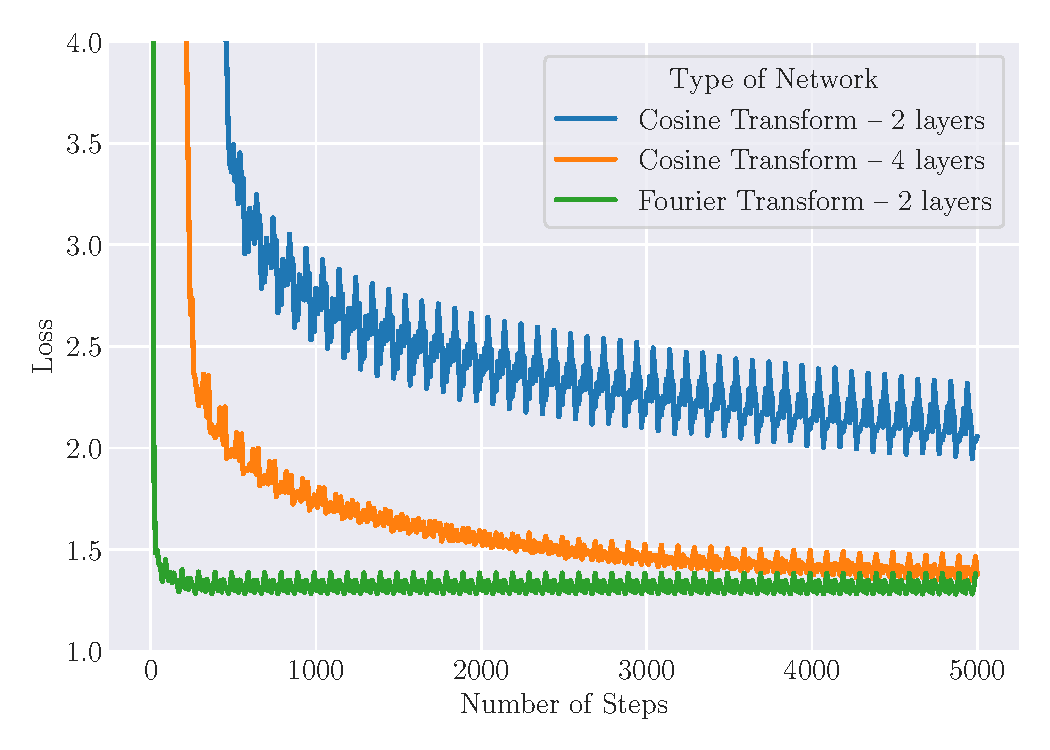
\includegraphics[width=\textwidth]{figures/main/ch4-diagonal_circulant/acdc_regression.pdf}
       \caption{Evolution of the training loss on a regression task with synthetic data.}
       \label{figure:p1-ch4-acdc_regression}
   \end{subfigure}
   \hfill
   \begin{subfigure}[b]{0.49\textwidth}
       \centering
       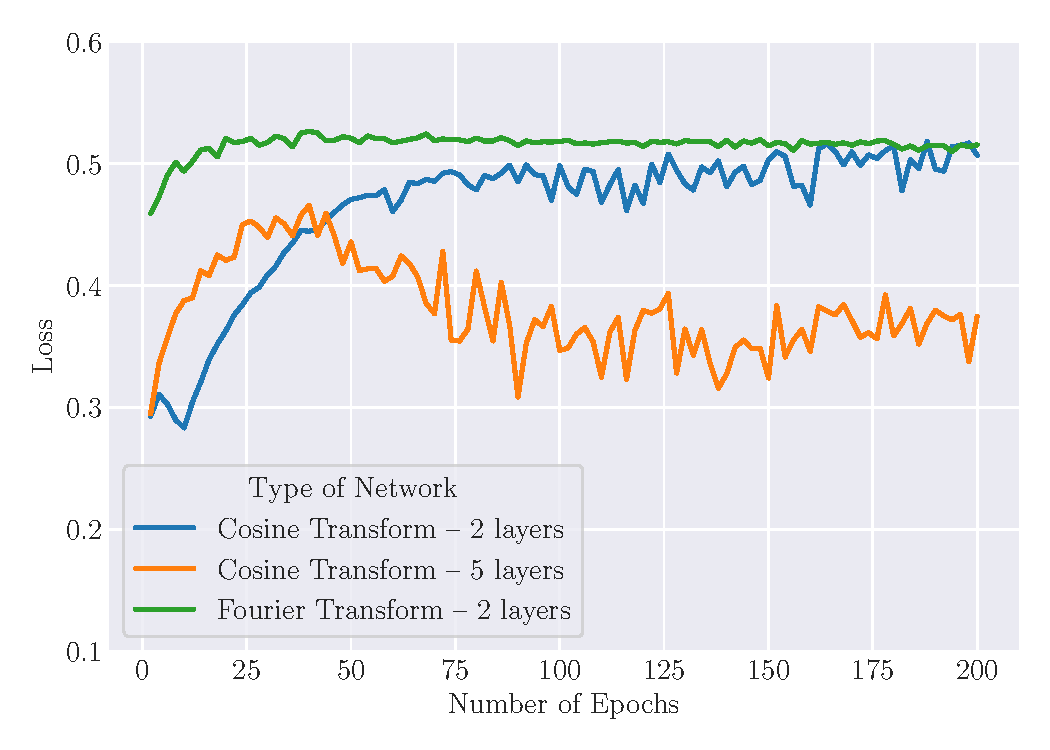
\includegraphics[width=\textwidth]{figures/main/ch4-diagonal_circulant/acdc_cifar10.pdf}
       \caption{Test accuracy on the CIFAR-10 dataset.~\\ \phantom{.}}
       \label{figure:p1-ch4-acdc_cifar10}
   \end{subfigure}
   \caption{Comparison of DCNNs and \ACDC networks on two different tasks.}
\end{figure}


\paragraph{Comparison with \ACDC \citep{moczulski2016acdc}.}

In Section~\ref{chapter:p1-ch3-related_work}, we have discussed the differences between the \ACDC framework and our approach from a theoretical perspective.
In this section, we conduct experiments to compare the performance of DCNNs with neural networks based on \ACDC layers. 
We first reproduce the experimental setting from \citet{moczulski2016acdc}, and compare both approaches using only linear networks (\ie networks without any ReLU activations).
The synthetic dataset has been created in order to reproduce the experiment on the regression linear problem proposed by~\citet{moczulski2016acdc}.
We draw $\Xmat$ and $\Wmat$ from a uniform distribution between [-1, +1] and $\epsilon$ from a normal distribution with mean 0 and variance $0.01$.
The relationship between $\Xmat$ and $\Ymat$ is define by $\Ymat = \Xmat\Wmat + \epsilon$. 
The results are presented in Figure~\ref{figure:p1-ch4-acdc_regression}.
On this simple setting, while both architectures demonstrate good performance, we can observe that DCNNs offer a better convergence rate.
In Figure~\ref{figure:p1-ch4-acdc_cifar10}, we compare neural networks with ReLU activations on CIFAR-10. 

We found that networks which are based only on \ACDC layers are difficult to train and offer poor accuracy on CIFAR-10 (we have tried different initialization schemes including the one from the original paper, and the one we introduce in this chapter).
\citet{moczulski2016acdc} manage to train a large VGG network  however these networks are generally highly redundant and the contribution of the structured layer is difficult to quantify. 
We also observe that adding a single dense layer improves the convergence rate of \ACDC in the linear case, which explains the good results of \citet{moczulski2016acdc}.
However, it is difficult to characterize the true contribution of the \ACDC layers when the network has a large number of expressive layers.

In contrast, deep DCNNs can be trained and offer good performance without additional dense layers (these results are in line with our experiments on the \yt dataset).
We can conclude that DCNNs are able to model complex relations at a low cost. 

\begin{figure}
   \centering
   \begin{tikzpicture}[scale=0.8]
\begin{axis}[
    legend cell align={left},
    xlabel={\large \#weights (x1000) },
    ylabel={Test Accuracy},
    xmin=21, xmax=370,
    ymin=0.2, ymax=0.6,
    legend pos=south east,
    ymajorgrids=true,
    grid style=dashed,
	]
    \addplot[color=red, line width=0.25mm, dashed] table [y=accuracy, x=weights]
    {figures/main/ch4-diagonal_circulant/data/cifar10/type/dense.dat};
    \addplot[mark=triangle, color=blue, line width=0.4mm] table [y=accuracy, x=weights]
    {figures/main/ch4-diagonal_circulant/data/cifar10/type/circulant.dat};
    \addplot[mark=square, color=red, line width=0.4mm] table [y=accuracy, x=weights]
    {figures/main/ch4-diagonal_circulant/data/cifar10/type/diag_toeplitz.dat};
    \addplot[mark=o, color=gray, line width=0.4mm] table [y=accuracy, x=weights]
    {figures/main/ch4-diagonal_circulant/data/cifar10/type/toeplitz.dat};
    \addplot[mark=diamond, color=brown, line width=0.4mm] table [y=accuracy, x=weights]
    {figures/main/ch4-diagonal_circulant/data/cifar10/type/low_rank.dat};
    \legend{
      Dense (9M weights),
      DCNN,
      DTNN,
      Toeplitz network,
      Low Rank network, 
     }
\end{axis}
\end{tikzpicture}

   \caption{Network size vs. Accuracy compared on Dense networks, DCNNs (our approach), DTNNs (our approach), neural networks based on Toeplitz matrices and neural networks based on Low Rank-based matrices. DCNNs outperforms alternatives structured approaches.}
   \label{figure:p1-ch4-cifar10_type}
\end{figure}

\begin{figure}
   \centering
   \begin{tikzpicture}[scale=0.8]
\begin{axis}[
    xlabel={\large \#weights (x1000) },
    ylabel={Test Accuracy},
    legend pos=outer north east,
    legend cell align={left},
    ymajorgrids=true,
    grid style=dashed,
    ]
    % \addplot[mark=oplus*,blue] coordinates {(15, 0.6178)}; % Random Conv + Dense
    % \addplot[mark=oplus*,red] coordinates {(90, 0.8438)}; % Conv + Dense
    \addplot[mark=triangle*,blue] coordinates {(140, 0.7017)}; % ldr-sd (rank=1)
    \addplot[mark=triangle*,red] coordinates {(420, 0.7286)}; % ldr-sd (rank=10)
    \addplot[mark=diamond*,blue] coordinates {(110, 0.7111)}; % toeplitz-like (rank=1)
    \addplot[mark=diamond*,red] coordinates {(388, 0.7205)}; % toeplitz-like (rank=10)
    \addplot[mark=square*,green] coordinates {(124, 0.757)}; % Scattering + 1 DC
    \addplot[mark=square*,blue] coordinates {(217, 0.7856)}; % Scattering + 3 DC
    \addplot[mark=square*,red] coordinates {(66, 0.7535)}; % Scattering Avg pooling + 3 DC
    \addplot[mark=square*,brown] coordinates {(191, 0.764)}; % Scattering by channel + 4 DC
    % \addplot[mark=square*,green] coordinates {(131, 0.704)}; % Conv 32 + Max Pooling + 5 DC
    \legend{
        % Random Conv + Dense,
        % Conv + Dense,
        Scattering + LDR-SD (r=1),
        Scattering + LDR-SD (r=10),
        Scattering + Toeplitz-like (r=1),
        Scattering + Toeplitz-like (r=10),
        Scattering + 1 DC,
        Scattering + 3 DC,
        Scattering Avg pooling + 3 DC,
        Scattering by channel + 4 DC,
        % Conv + Max Pooling + DC,
    }
\end{axis}
\end{tikzpicture}

		

   \caption{Accuracy of different structured architecture given the number of trainable parameters.}
   \label{figure:p1-ch4-cifar10_with_channels_xp}
\end{figure}


\paragraph{Comparison with Dense networks, Toeplitz networks and Low Rank networks.}
We now compare DCNNs with other state-of-the-art structured networks by measuring the accuracy on a flattened version of the CIFAR-10 dataset.
Our baseline is a dense feed-forward network with a fixed number of weights (9 million weights).
We compare with DCNNs and with DTNNs (see below), Toeplitz networks, and Low-Rank networks~\cite{yu2017compressing}.
We first consider Toeplitz networks which are stacked Toeplitz matrices interleaved with ReLU activations since Toeplitz matrices are closely related to circulant matrices.
However, Toeplitz networks have a different structure than DCNNs (they do not include diagonal matrices), therefore, we also experiment using DTNNs, a variant of DCNNs where all the circulant matrices have been replaced by Toeplitz matrices.
Finally we conduct experiments using networks based on low-rank matrices as they are also closely related to our work.
For each approach, we report the accuracy of several networks with a varying depth ranging from 1 to 40 (DCNNs, Toeplitz networks) and from 1 to 30 (from DTNNs).
For low-rank networks, we used a fixed depth network and increased the rank of each matrix from 7 to 40.
We also tried to increase the depth of low rank matrices, but we found that deep low-rank networks are difficult to train so we do not report the results here.
We compare all the networks based on the number of weights from 21K (0.2\% of the dense network) to 370K weights (4\% of the dense network) and we report the results in Figure~\ref{figure:p1-ch4-cifar10_type}. 
First we can see that the size of the networks correlates positively with their accuracy which demonstrate successful training in all cases.
We can also see that the DCNNs achieves the maximum accuracy of 56\% with 20 layers ($\sim$ 200K weights) which is as good as the dense networks with only 2\% of the number of weights.
Other approaches also offer good trade-off but they are not able to reach the accuracy of a dense network.


\begin{table}[htb]
  \centering
  \begin{tabular}{lcc}
    \toprule
    \textbf{Architectures} & \textbf{\#Params} & \textbf{Acc.}  \\
    \midrule
    \textit{Dense} & \textit{9.4M}	& \textit{0.562} \\
    \textbf{\textit{DCNN $(5\ layers)$}} & \textbf{49K}	& \textbf{0.543} \\
    \textbf{\textit{DCNN $(2\ layers)$}} & \textbf{21K} & \textbf{0.536} \\
    LDR--TD	$(r = 2)$	        & 64K	& 0.511 \\
    LDR--TD	$(r = 3)$	        & 70K	& 0.473 \\
    Toeplitz-like $(r=2)$	    & 46K	& 0.483 \\
    Toeplitz-like $(r =3)$	    & 52K    & 0.496 \\
    \bottomrule
    \end{tabular}
    \caption{LDR networks compared with DCNNs on a flattend version of CIFAR-10. DCNNs outperform all LDR configurations with fewer weights. Remark: the numbers may differ from the original experiments by~\citet{thomas2018learning} because we use the original dataset instead of a monochrome version.}
    \label{table:xp_ldr}
\end{table}

\begin{table}[htb]
  \centering
  \begin{tabular}{lcc}
    \toprule
    \textbf{Architectures} & \textbf{\#Params} & \textbf{Acc.}  \\
    \midrule
    \textbf{DC $(1\ layers)$} & \textbf{124K} & \textbf{0.757} \\
    \textbf{DC $(3\ layers)$} & \textbf{217K} & \textbf{0.785} \\
    \textbf{Ensemble x5 DC $(3\ layers)$} &  \textbf{1.08M} & \textbf{0.811} \\
    LDR-SD $(r=1)$ & 140K & 0.701 \\
    LDR-SD $(r=10)$ & 420K & 0.728 \\
    Toeplitz-like $(r=1)$ & 110K & 0.711 \\
    Toeplitz-like $(r=10)$ & 388K & 0.720 \\
    \bottomrule
    \end{tabular}
    \caption{Two depths scattering on CIFAR-10 followed by LDR or DC layer. Networks with DC layers outperform all LDR configurations with fewer weights.}
    \label{table:xp_ldr_scattering}
\end{table}


\paragraph{Comparison with LDR networks~\cite{thomas2018learning}.}
We now compare DCNNs with the LDR framework using the network configuration experimented in the original paper: a single LDR structured layer followed by a dense layer.
In the LDR framework, we can change the size of a network by adjusting the rank of the residual matrix, effectively capturing matrices with a structure that is close to a known structure but not exactly (in the LDR framework, Toeplitz matrices can be encoded with a residual matrix with rank=2, so a matrix that can be encoded with a residual of rank=3 can be seen as Toeplitz-like.).
The results are presented in Table~\ref{table:xp_ldr} and demonstrate that DCNNs outperforms all LDR networks both in terms in size and accuracy.

\paragraph{Exploiting image features.}
Dense layers and DCNNs are not designed to capture task-specific features such as the translation invariance inherently useful in image classification.
We can further improve the accuracy of such general purpose architectures on image classification without dramatically increasing the number of trained parameters by stacking them on top of fixed (ie non-trained) transforms such as the scattering transform \cite{mallat2010recursive}.
In this section we compare the accuracy of various structured networks, enhanced with the scattering transform, on an image classification task, and run comparative experiments on CIFAR-10. 

Our test architecture consists of 2 depth scattering on the RGB images followed by a batch norm and LDR or DC layer.
To vary the number of parameters of Scattering+LDR architecture, we increase the rank of the matrix (stacking several LDR matrices quickly exhausted the memory).
The Figure \ref{figure:p1-ch4-cifar10_with_channels_xp} and \ref{table:xp_ldr_scattering} shows the accuracy of these architectures given the number of trainable parameters.

First, we can see that the DCNN architecture very much benefits from the scattering transform and is able to reach a competitive accuracy over 78\%.
We can also see that scattering followed by a DC layer systematically outperforms scattering + LDR or scattering + Toeplitz-like with less parameters. 


%%%%%%%%%%%%%%%%%%%%%%%%%%%%%%%%%%%%%%%%%%%%%%%%%%%%%%%%%%%%%%%%%%%%%%%%%%%%%%%
\subsection{Comparison with other compression based approaches}
\label{subsection:p1-ch4-comparison_with_other_compression_based_approaches}
%%%%%%%%%%%%%%%%%%%%%%%%%%%%%%%%%%%%%%%%%%%%%%%%%%%%%%%%%%%%%%%%%%%%%%%%%%%%%%%


\begin{table}
  \centering
    \caption{Comparison with compression based approaches}
    \begin{tabular}{lcrc}
    \toprule
    \multicolumn{1}{c}{\textbf{Architecture}} & \multicolumn{1}{c}{\textbf{\#Params}} & \textbf{Error (\%)} \\
    \hline \\
    \textit{LeNet \cite{Lecun98gradient-basedlearning}} & \textit{4 257 674} & \textit{0.61} \\
    \multirow{2}[0]{*}{\textbf{DCNN}} & \textbf{25 620} & \textbf{1.74} \\
          & \textbf{31 764} & \textbf{1.60} \\
    \multirow{2}[0]{*}{HashNet \cite{chen2015compressing}} & 46 875 & 2.79 \\
          &  78 125 & 1.99 \\
    \multirow{2}[0]{*}{Dark Knowledge \cite{hinton2015distilling}} & 46 875 & 6.32 \\
          &  78 125 & 2.16 \\
    \bottomrule
    \end{tabular}%
  \label{tab:mnist}%
\end{table}%


We provide a comparison with other compression based approaches such as HashNet \cite{chen2015compressing}, Dark Knowledge \cite{hinton2015distilling} and Fast Food Transform (FF) \cite{yang2015deep}. 
Table~\ref{tab:mnist} shows the test error of DCNN against other know compression techniques on the MNIST datasets. We can observe that DCNN outperform easily HashNet \cite{chen2015compressing} and Dark Knowledge \cite{hinton2015distilling} with fewer number of parameters. The architecture with Fast Food (FF) \cite{yang2015deep} achieves better performance but with convolutional layers and only $1$ Fast Food Layer as the last Softmax layer. 


% %%%%%%%%%%%%%%%%%%%%%%%%%%%%%%%%%%%%%%%%%%%%%%%%%%%%%%%%%%%%%%%%%%%%%%%%%%%%%%%
% \subsection{Large-scale video classification on the \yt dataset}
% \label{subsection:p1-ch4-large_scale_video_classification}
% %%%%%%%%%%%%%%%%%%%%%%%%%%%%%%%%%%%%%%%%%%%%%%%%%%%%%%%%%%%%%%%%%%%%%%%%%%%%%%%
%
% To understand the performance of deep DCNNs on large scale applications, we conducted experiments on the \yt video classification with 3.8 training examples introduced by~\citet{abu2016youtube}.
% Notice that we favour this experiment over ImageNet applications because modern image classification architectures involve a large number of convolutional layers, and compressing convolutional layers is out of our scope. 
% Also, as mentioned earlier, testing the performance of DCNN architectures mixed with a large number of expressive layers makes little sense.
% The \yt includes two datasets describing 8 million labeled videos.
% Both datasets contain audio and video features for each video.
% In the first dataset (\emph{aggregated}) all audio and video features have been aggregated every 300 frames.
% The second dataset (\emph{full}) contains the descriptors for all the frames.
% To compare the models we use the GAP metric (Global Average Precision) proposed by~\citet{abu2016youtube}.
% On the simpler \emph{aggregated} dataset we compared off-the-shelf DCNNs with a dense baseline with 5.7M weights.
% On the full dataset, we designed three new compact architectures based on the state-of-the-art architecture introduced by~\citet{abu2016youtube}. 
%
% \paragraph{Experiments on the aggregated dataset with DCNNs:}
% We compared DCNNs with a dense baseline with 5.7 millions weights.
% The goal of this experiment is to discover a good trade-off between depth and model accuracy.
% To compare the models we use the GAP metric (Global Average Precision) following the experimental protocol in~\cite{abu2016youtube}, to compare our experiments. 
%
% Table~\ref{table:youtube_agg_xp} shows the results of our experiments on the {\em aggrgated} \yt dataset in terms of number of weights, compression rate and GAP.
% We can see that the compression ratio offered by the circulant architectures is high.
% This comes at the cost of a little decrease of GAP measure.
% The 32 layers DCNN is 46 times smaller than the original model in terms of number of parameters while having a close performance. 
%
%
% \begin{table}
%   \centering
%   \caption{This table shows the GAP score for the \yt dataset with DCNNs. We can see a large increase in the score with deeper networks.}
%   \begin{tabular}{lccc}
%     \toprule
%     \textbf{Architecture} & \textbf{\#Weights} &
%     \textbf{GAP@20} \\
%     \hline \\
%     \textit{original} & \textit{5.7M} & \textit{0.773} \\
%     4 DC & 25 410  (\textit{\textbf{0.44}}) & 0.599   \\
%     32 DC  & 122 178 \textit{(2.11)} & 0.685   \\
%     4 DC + 1 FC & 4.46M \textit{(77)} & \textbf{0.747} \\
%   \hline
%   \end{tabular}
%   \label{table:youtube_agg_xp}
% \end{table}
%
% \begin{table}
%   \centering
%   \caption{This table shows the GAP score for the \yt dataset with different layer represented with our DC decomposition.}
%   \begin{tabular}{lccc}
%   \toprule
%   \textbf{Architecture} & \textbf{\#Weights} & \textbf{GAP@20} \\
%   \hline \\
%   \textit{original} & \textit{45M} & \textit{0.846} \\
%   DBoF with DC   & 36M (\textit{80}) & 0.838 \\
%   FC with DC    & 41M (\textit{91}) & \textbf{0.845} \\
%   MoE with DC   & 12M (\textit{\textbf{26}}) & 0.805 \\
%   \hline
%   \end{tabular}
%   \label{table:youtube_full_xp}
% \end{table}
%
% \paragraph{Experiments with DCNNs Deep Bag-of-Frames Architecture:}
% The Deep Bag-of-Frames architecture can be decomposed into three blocks of layers, as illustrated in Figure~\ref{figure:p1-ch4-archi_youtube}.
% The first block of layers, composed of the Deep Bag-of-Frames embedding (DBoF), is meant to model an embedding of these frames in order to make a simple representation of each video.
% A second block of fully connected layers (FC) reduces the dimensionality of the output of the embedding and merges the resulting output with a concatenation operation.
% Finally, the classification block uses a combination of Mixtures-of-Experts (MoE)~\cite{jordan1993hierarchical,abu2016youtube} and Context Gating~\cite{miech2017learnable} to calculate the final class probabilities.
% Table~\ref{table:youtube_full_xp} shows the results in terms of number of weights, size of the model (MB) and GAP on the full dataset, replacing the DBoF block reduces the size of the network without impacting the accuracy.
% We obtain the best compression ratio by replacing the MoE block with DCNNs (26\%) of the size of the original dataset with a GAP score of 0.805 (95\% of the score obtained with the original architecture).
% We conclude that DCNN are both theoretically sound and of practical interest in real, large scale applications.
%
% \begin{figure}[htb]
%   \centering
%   \tikzset{%
  >={Latex[width=2mm,length=2mm]},
  % Specifications for style of nodes:
            base/.style = {rectangle, draw=black, text centered, font=\sffamily},
             box/.style = {base, rounded corners, text depth=3cm, minimum height=4cm, minimum width=3cm},
     transparent/.style = {rectangle, draw=black},
       circulant/.style = {base, fill=yellow!30},
       embedding/.style = {base, fill=blue!30, minimum width=2.5cm, minimum height=1cm},
           other/.style = {base, fill=white!30,  minimum width=2cm, minimum height=1cm},
              fc/.style = {base, fill=orange!30, minimum width=1.5cm, minimum height=1cm},
          gating/.style = {base, fill=green!30, minimum width=2cm, text width=2cm, minimum height=1cm},
             moe/.style = {base, fill=purple!30, minimum width=1.5cm, minimum height=1cm},
}

\begin{tikzpicture}[every node/.style={fill=white, font=\sffamily}, align=center]

  \draw (0.0, +2.)  node [other, draw=none] {\textbf{Embedding}};
  \draw (+3.7, +2.)  node [other, draw=none] {\textbf{Dim Reduction}};
  \draw (+8.0, +2.)  node [other, draw=none] {\textbf{Classification}};

  \draw (0, +0.8)  node [embedding] {Video};
  \draw (0, -0.8)  node [embedding] {Audio};

  \draw (+2.5, +0.8)  node (fc) [fc] {FC};
  \draw (+2.5, -0.8)  node (fc) [fc] {FC};

  \draw (+4.75, 0)  node (fc) [other] {concat};
  \draw (+7.0, 0)  node (moe) [moe] {MoE};
  \draw (+9.25, 0)  node (gating2) [gating] {Context Gating};
 
  \draw (+1.5, +2) [dashed] -- (+1.5, -1.7);
  \draw (+6, +2) [dashed] -- (+6, -1.7);
  
\end{tikzpicture}

%   \caption{This figure shows the state-of-the-art neural network architecture, initially proposed by~\citet{abu2016youtube} and later improved by~\citet{miech2017learnable}, used in our experiment.}
%   \label{figure:p1-ch4-archi_youtube}
% \end{figure}
%
% \paragraph{Architectures \& Hyper-Parameters:} 
% For the first set of our experiments (\emph{experiments on CIFAR-10}), we train all networks for 200 epochs, a batch size of 200, Leaky ReLU activation with a different slope.
% We minimize the Cross Entropy Loss with Adam optimizer and use a piecewise constant learning rate of $5 \times 10^{-5}$, $2.5\times10^{-5}$, $5\times10^{-6}$ and $1\times10^{-6}$ after respectively 40K, 60K and 80K steps.
% For the \yt dataset experiments, we built a neural network based on the SOTA architecture initially proposed by~\citet{abu2016youtube} and later improved by~\citet{miech2017learnable}.
% Remark that no convolution layer is involved in this application since the input vectors are embeddings of video frames processed using state-of-the-art convolutional neural networks trained on ImageNet.
% We trained our models with the CrossEntropy loss and used Adam optimizer with a 0.0002 learning rate and a 0.8 exponential decay every 4 million examples.
% All fully connected layers are composed of 512 units.
% DBoF, NetVLAD and NetFV are respectively 8192, 64 and 64 of cluster size for video frames and 4096, 32, 32 for audio frames.
% We used 4 mixtures for the MoE Layer.
% We used all the available 300 frames for the DBoF embedding.
% In order to stabilize and accelerate the training, we used batch normalization before each non linear activation and gradient clipping. 

% %%%%%%%%%%%%%%%%%%%%%%%%%%%%%%%%%%%%%%%%%%%%%%%%%%%%%%%%%%%%%%%%%%%%%%%%%%%%%%%
% \section{Conclusion}
% \label{section:p1-ch4-conclusion}
% %%%%%%%%%%%%%%%%%%%%%%%%%%%%%%%%%%%%%%%%%%%%%%%%%%%%%%%%%%%%%%%%%%%%%%%%%%%%%%%

% This chapter deals with the training of diagonal circulant neural networks.
% To the best of our knowledge, training such networks with a large number of layers had not been done before.
% We also endowed this kind of models with theoretical guarantees, hence enriching and refining previous theoretical work from the literature.
% More importantly, we showed that DCNNs outperform their competing structured alternatives, including the very recent general approach based on LDR networks.
% Our results suggest that stacking diagonal circulant layers with non linearities improves the convergence rate and the final accuracy of the network.
% Formally proving these statements constitutes the future directions of this work.
% We would like to generalize the good results of DCNNs to convolutional neural networks.
% We also believe that circulant matrices deserve a particular attention in deep learning because of their strong ties with convolutions: a circulant matrix operator is equivalent to the convolution operator with circular paddings.
% This fact makes any contribution to the area of circulant matrices particularly relevant to the field of deep learning with impacts beyond the problem of designing compact models.
% As future work, we would like to generalize our results to deep convolutional neural networks. 


